\documentclass[tikz,border=10pt]{standalone}
\usepackage{tikz}
\begin{document}
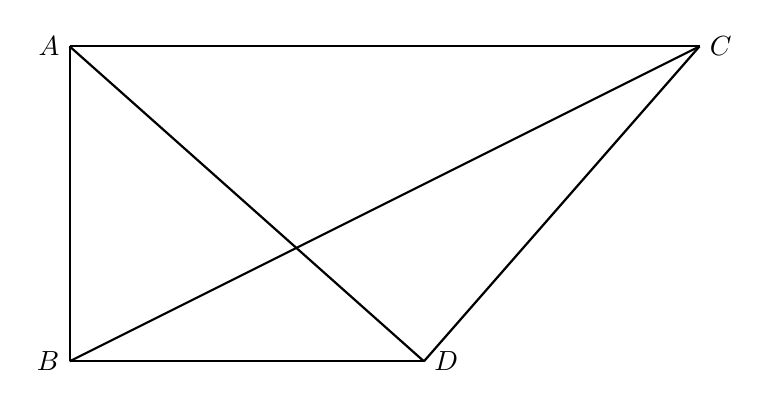
\begin{tikzpicture}[thick]
  \coordinate (A) at (0,4);
  \coordinate (B) at (0,0);
  \coordinate (C) at (8,4);
  \coordinate (D) at (4.5,0);

  \draw (A) -- (C);
  \draw (A) -- (B);
  \draw (B) -- (D);
  \draw (A) -- (D);
  \draw (B) -- (C);
  \draw (D) -- (C);

  \node[left] at (A) {$A$};
  \node[left] at (B) {$B$};
  \node[right] at (C) {$C$};
  \node[right] at (D) {$D$};
\end{tikzpicture}
\end{document}
